% ===========================================
% Learning Materials and Set Up
% Written by: Braidan Duffy
%
% Date: 06/13/2022
% Last Revision: 06/13/2022
% ============================================

\chapter*{Learning Materials and Setup}
\setchapterpreamble[u]{\margintoc}
\labch{b1_learning_materials}
\addcontentsline{toc}{chapter}{Learning Materials and Setup} % Add the preface to the table of contents as a chapter

This course will require you to become familiar with different software packages and get you hands on with real-world electronics hardware.
In this chapter, we will go into the required course material and give you an overview of what it is, how to set it up, and what you will be expected to know.

These are for your reference, so please follow these instructions closely and pay attention to the component overview parts so you can have more time playing and experimenting than troubleshooting.

\section*{Autodesk Fusion 360}
This is some test content

\section*{Arduino Kit Introduction}
You will all be required to purchase an Arduino learning kit. 
It is highly recommended you purchase the Arduino Mega complete starter kit from ELEGOO as it has all of the components necessary for the course, as well as a multitude of projects for your own education.
Additionally, the expansive IO of the Arduino Mega will make certain projects easier for you through the course and give you larger amounts of program storage and memory for more complex projects.

Most of the simpler discreet parts will be discussed ad nausiem in later sections of these notes.
Therefore, they will be skipped in this section.
Below are some of the more unique parts of the Arduino Mega kit and what they can do.
    
    \subsection*{Microcontroller}
    The Arduino Mega uses an ATmega2560 microcontroller to execute programs and interface with a wide variety of inputs and outputs.\marginnote{More information on the Arduino Mega can be found the Arduino website - \url{https://www.arduino.cc/en/Guide/ArduinoMega2560/}}
    This chip has:
    \begin{itemize}
        \item 86 programmable General Purpose Input/Output (GPIO) pins that operate at a 5V TTL logic.
        \item 16 10-bit analog inputs
        \item 2 8-bit counters; 2 16-bit counters
        \item 1 Serial Peripheral Interface (SPI) bus
        \item 4 Universal Synchronous/Asynchronous Receive/Transmit (USART) busses
        \item 256 KB of flash memory for program storage
        \item 8 KB of SRAM for program memory
        \item 8 KB of EEPROM for long term, fast access storage
    \end{itemize}

    The ATmega2560 has been widely adopted by the Arduino and maker community so there is rich and mature development support for the chip.
    In this course, you will be using the Arduino IDE (or Visual Studio Code) to program the microntroller. 
    Normally, flashing code to a microntroller is not a streamlined process, but thanks to the hard work on the Arduino Foundation and a globe-spanning community, all that is required to go from code to a blinking light is a USB cable and the push of a button.

    \begin{figure*}[h!]
        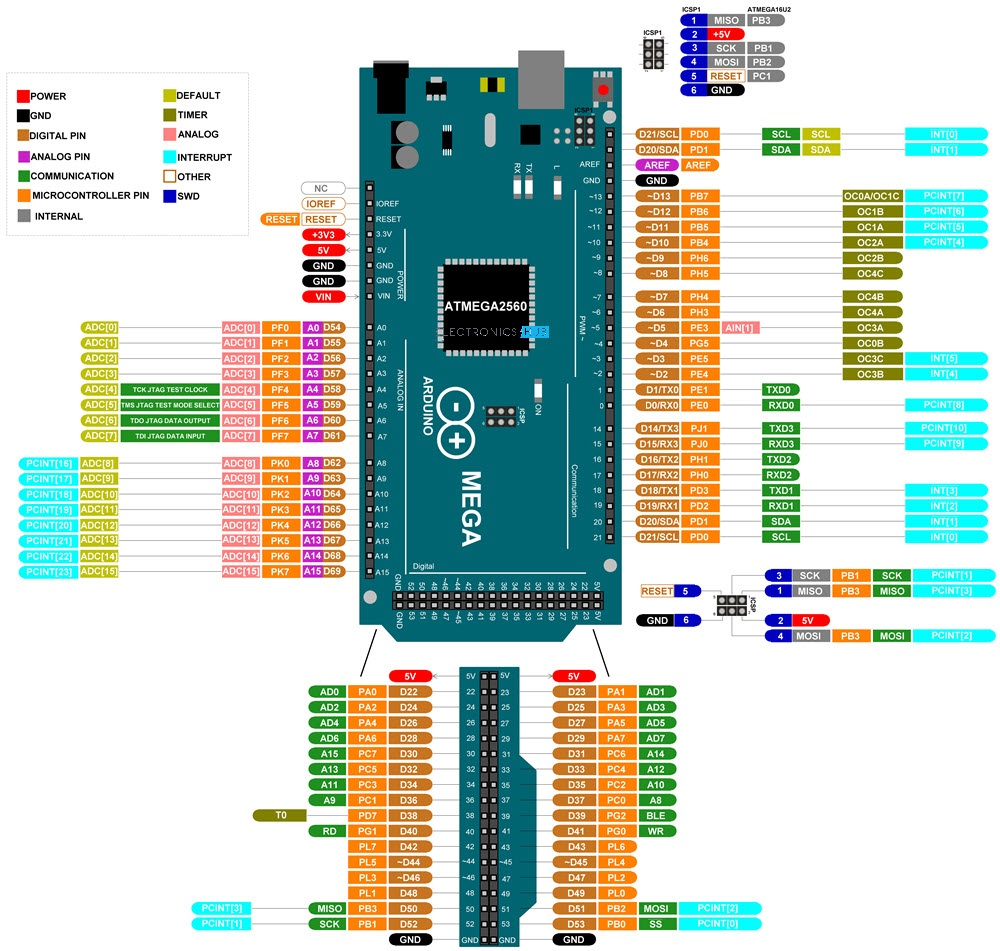
\includegraphics[height=6in]{learning_materials/Arduino-Mega-Pinout.jpg}
        \caption[Arduino Mega Pinout]{The pinout for the Arduino Mega. Retreived from \href{https://www.electronicshub.org/wp-content/uploads/2021/01/Arduino-Mega-Pinout.jpg}{Electronics Hub}}
        \labfig{arduino_mega_pinout}
    \end{figure*}

    \subsection*{MAX7219 LED Matrix Module}
    The MAX7219 is a common cathode LED driver IC that has a four wire serial interface compatible with all microcontrollers.
    The IC is capable of driving up to 64 LEDs making it perfect for driving dot matrix displays and 7-segment displays.
    It also has a built-in BCD decoder and 64-byte static RAM which makes it very easy to display numbers, letters, or symbols on a dot matrix or 7-segment display.

    \begin{figure}[h!]
        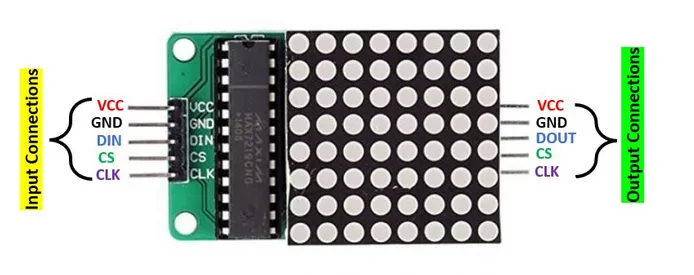
\includegraphics[]{learning_materials/MAX7219-led-matrix-pin-out.png}
        \caption[LED Matrix Pinout]{The pinout for the 8x8 LED dot matrix present in the Arduino Mega Starter Kit. 
        Retreived from \href{https://microcontrollerslab.com/wp-content/uploads/2021/09/MAX7219-led-matrix-pin-out.jpg?ezimgfmt=ng:webp/ngcb1}{Microcontrollers Lab}}
        \labfig{led_matrix_pinout}
    \end{figure}

    \marginnote{Additional information on the MAX7219 can be found here: \url{https://microcontrollerslab.com/max7219-8-digit-led-display-driver/}}

    For this particular kit, the MAX7219 drives an LED dot matrix with 8 rows and 8 columns (64 LEDs total). 
    Each LED is addressible by its particular row and column number.
    As seen in Figure \ref{fig:led_matrix_schematic}, the positive terminal of the LED "dot" is connected to a row pin, and the negative terminal of the dot is connected to a column pin.
    By setting a particular row to a positive voltage and a particular column to ground, we can turn on a dot.
    This matrix layout is a form of multiplexing and allows a microcontroller to drive 64 LEDs with only 16 pins!

    \begin{figure}[b!]
        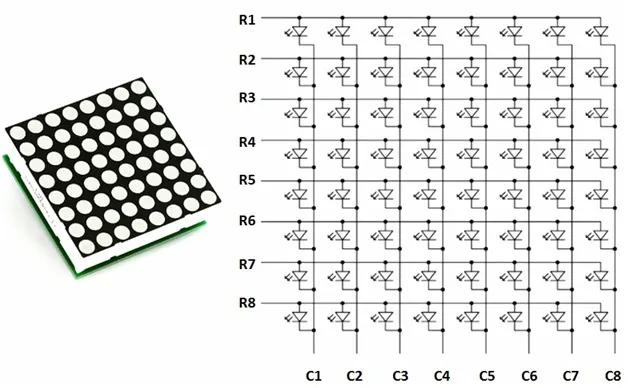
\includegraphics[height=3in]{learning_materials/led-matrix.png}
        \caption[LED Matrix Schematic]{The schematic for the 8x8 LED dot matrix present in the Arduino Mega Starter Kit. 
        Retreived from \href{https://microcontrollerslab.com/wp-content/uploads/2016/11/led-matrix.jpg?ezimgfmt=ng:webp/ngcb1}{Microcontrollers Lab}}
        \labfig{led_matrix_schematic}
    \end{figure}

    However, 16 pins is still a substantial amount for an embedded platform and computing the logic for which LEDs to turn on/off for a specific symbol wastes valuable compute cycles.
    It is much more efficient for us to use a dedicated IC like the MAX7219 to handle driving the matrix for us. 
    The IC can use its built-in serial decoder to drive all 64 LEDs from 4 pins on the microcontroller.
    It also handles all of the logic for displaying specific symbols, releiving the microcontroller from additional calculations.
    Since the MAX7219 sole purpose is to drive LED displays, it can also run much faster allowing programs to display text that smoothly scrolls across the matrix with minimal interruption.
    
    The MAX7219 serial bus also supports daisy chaining so multiple LED matrices can be connected in series to make a larger overall display.\sidenote{This does come at the cost of increasing input delay with every module. Too many modules chained together can have undesirable performance.}

    \subsection*{DS3231 Real-time Clock Module}
    The DS3231 is a sophisticated real-time clock module that maintains a high time keeping accuracy over a long period of time and a range of temperatures.
    You can communicate with the DS3231 over the I2C bus which makes it extremely simple to get up and running with most microcontrollers.
    It also has a low power draw so it can be powered by a dedicated battery to ensure that projects have an accurate time keeper for data-logging, wake up interrupts, etc.

    Once you initialize the date and time on the module, you will be able to routinely get the day, month, year, day of the week, hour, minute, and second from the IC over I2C. So long as it has power, it will provide you the time.

    \begin{figure}[h]
        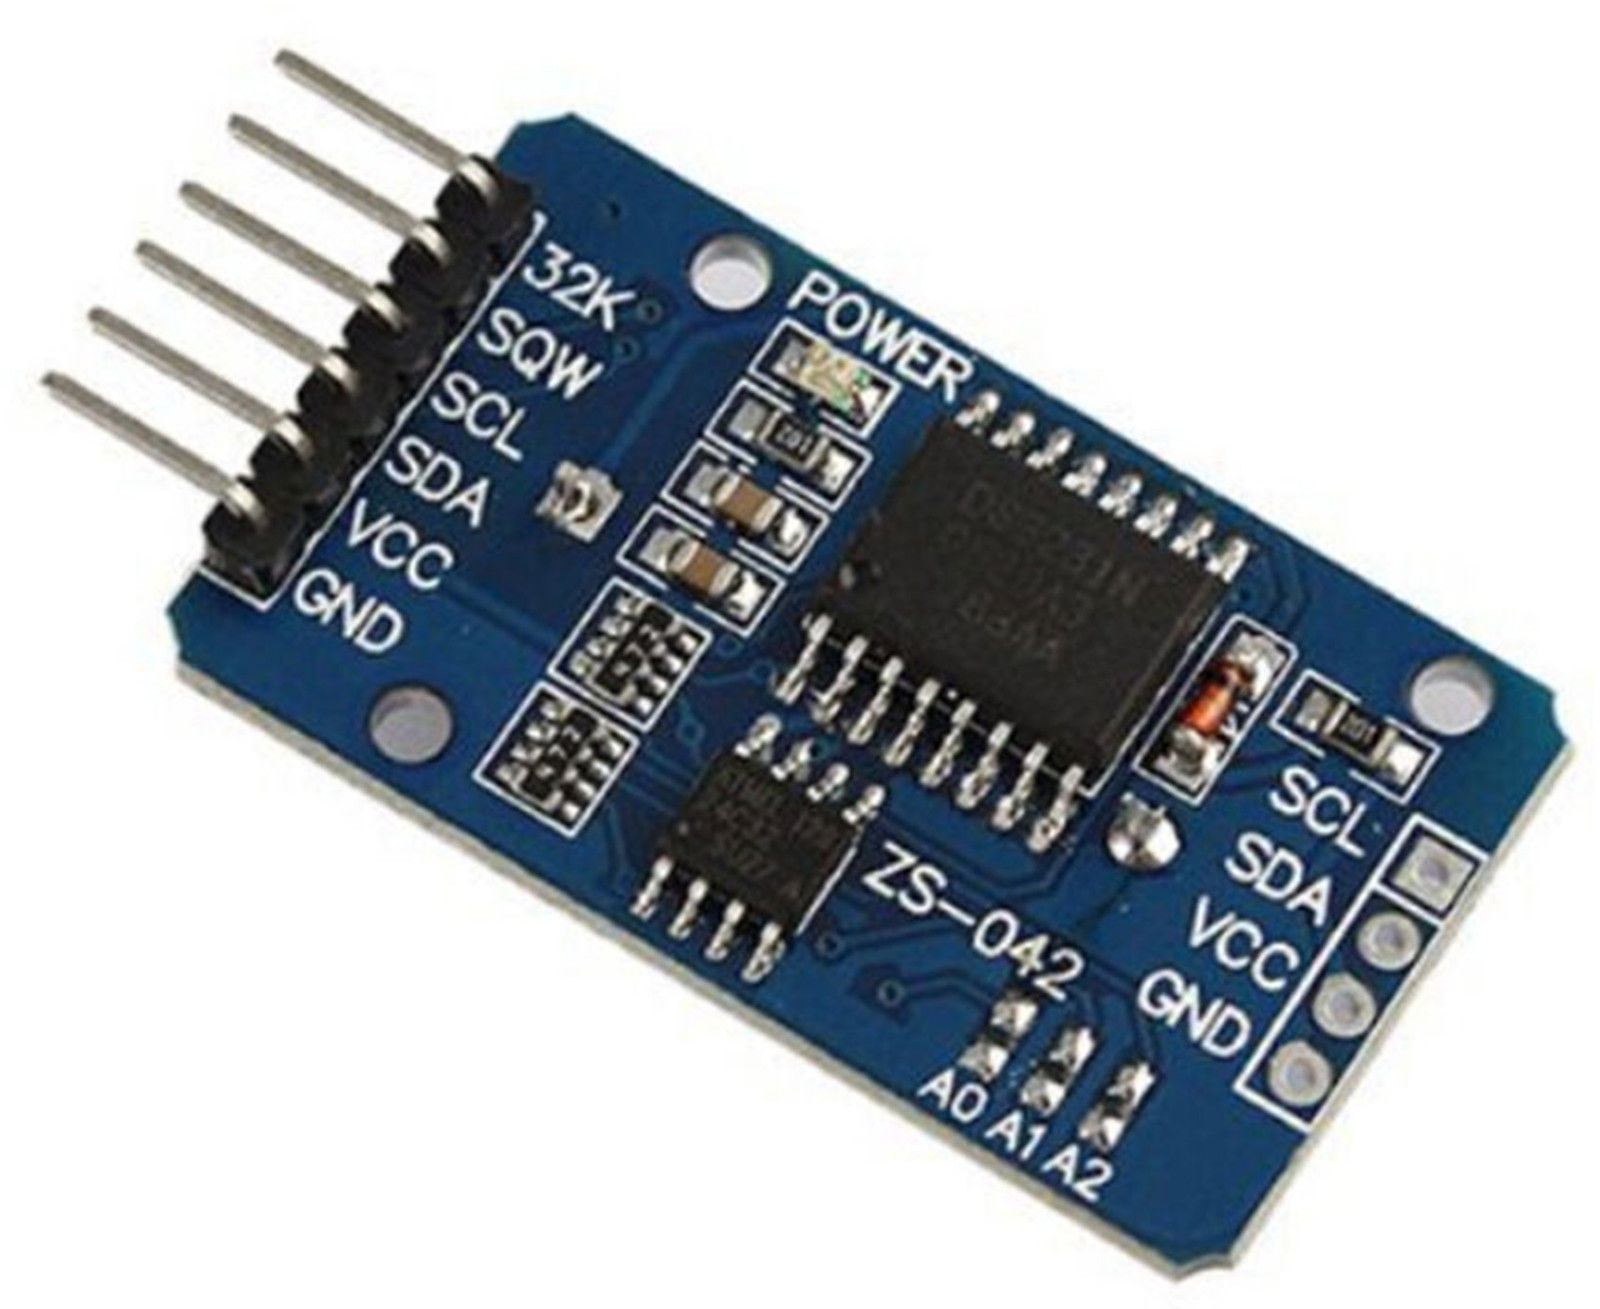
\includegraphics[height=2.5in]{learning_materials/ds3231-rtc.jpg}
        \caption[DS3231 RTC Module]{The DS3231 RTC module from the Arduino kit. 
        Retreived from \href{https://alltopnotch.co.uk/wp-content/uploads/imported/9/RTC-Real-Time-Clock-DS3231-I2C-AT24C32-Board-Module-Arduino-ARM-PIC-UK-Seller-361515587149-4.JPG}
        {All Top Notch}}
        \labfig{ds3231_rtc}
    \end{figure}

    \subsection*{Matrix Keypad}
    The ELEGOO kit comes with a 4x4 matrix keypad with 16 individual keys.
    Much like the LED dot matrix, the keypad multiplexes the 16 buttons into four row pins, and four column pins, as shown in Figure \ref{fig:matrix_keypad}.
    In order to use the keypad, you will "scan" the matrix by connecting each column pin to an input with a pullup resistor, and each row to an output pin.
    By incrementally setting each row pin to low, and checking the input of each column pin, you can determine which button has been pressed.
    For example, if you are checking the second row of buttons by setting that pin to low and the third column pin is also low, than the button in position (2,3) (normally `6') is pressed.

    \begin{figure}[h]
        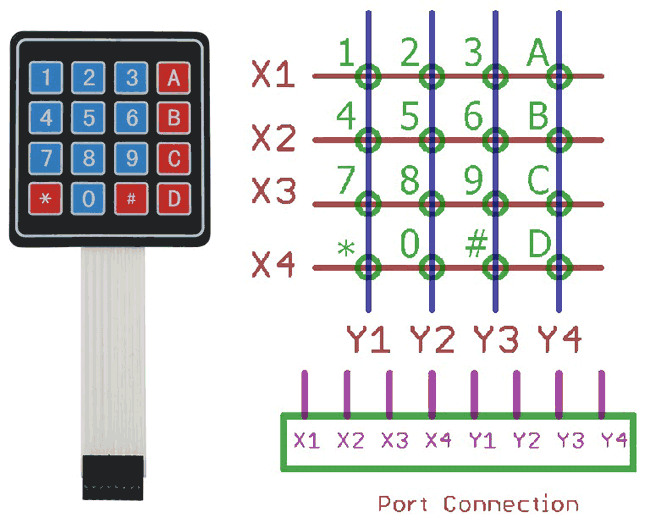
\includegraphics[height=2.5in]{learning_materials/4x4-matrix-keypad.png}
        \caption[4x4 Matrix Keypad]{The pinout and schematic for the 4x4 matrix keypad included in the Arduino starter kit. 
        Retreived from \href{https://dhaneshablogs.blogspot.com/2019/08/interfacing-4x4-matrix-keypad-with.html}
        {Dhanesha Blogs}}
        \labfig{matrix_keypad}
    \end{figure}

    \subsection*{PIR Motion Sensor}
    Passive Infrared (PIR) motion sensors detect levels of infrared radiation in their field of view.
    Inside a plastic bubble housing is a crystal that is sensative to IR radiation and is split into two halves.
    If one half of the crystal detects a different level of IR radiation than the other, the PIR driver IC will trigger a change on the interrupt line.
    This allows a microcontroller to do basic human sensing applications for monitoring foot traffic in an area, or if someone has entered/left a room.
    Additionally, the PIR sensor has some potentiometers that allow users to tweak the sensativity of the module and the time delay between triggers.

    \begin{figure}[h]
        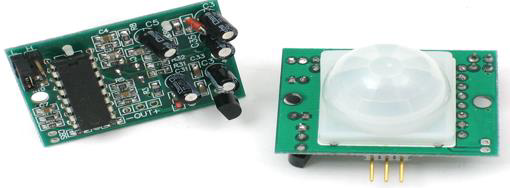
\includegraphics[height=2.5in]{learning_materials/pir_sensor.jpg}
        \caption[PIR Sensor]{The PIR sensor module included in the Arduino kit. 
        Retreived from \href{https://www.tutorialspoint.com/arduino/arduino_pir_sensor.htm}
        {Tutorials Point}}
        \labfig{matrix_keypad}
    \end{figure}

    \subsection*{IR Receiver}
    The IR receiver opreates with the same physical principles as the PIR motion sensor, but has much simpler circuitry.
    Inside a small housing is a crystal that is sensative to IR radiation.
    When the crystal is excited, it creates an electrical signal that can be read by a microcontroller on the output pin.
    All IR remotes (including the one in yyour Arduino kit) encode your button presses as flashes of IR light.
    When the IR receiver "sees" these flashes, it will convert them to an electrical signal with roughly the same timing as the remote output.
    This allows you to communicate with your microcontroller over light waves and signal it for different actions or functions. 
    \marginnote{This is the same exact way older TVs and AV receivers and DVD players function. 
    Pressing a button on your remote would send an encoded signal to turn up or down the volume, change the channel, or fast forward a movie.
    Universal remotes simply were able to switch between different encoding schema for different devices.
    Can you decode the messages your TV receives?}

    \begin{figure}[h]
        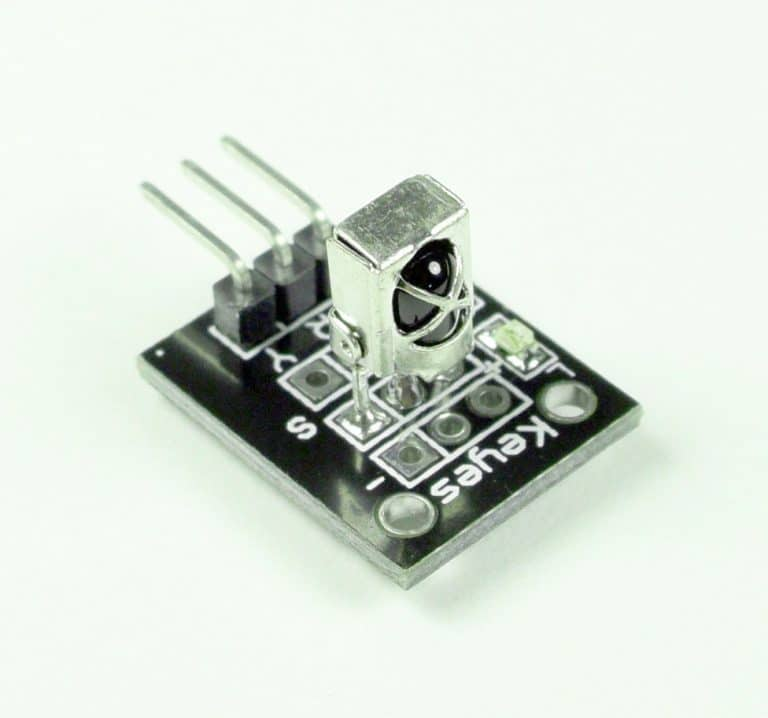
\includegraphics[height=2.5in]{learning_materials/ir-receiver.jpg}
        \caption[IR Receiver]{The IR receiver module included in the Arduino kit. 
        Retreived from \href{https://www.circuitbasics.com/arduino-ir-remote-receiver-tutorial/}
        {Circuit Basics}}
        \labfig{ir_receiver}
    \end{figure}

    \subsection*{LCD Screen}


    \subsection*{Joystick}


    \subsection*{Ultrasonic Distance Sensor}


    \subsection*{Sound Receiver}


    \subsection*{ULN2003 Motor Driver Board}


    \subsection*{DHT-11 Sensor}


    \subsection*{Capacitive Level Sensor}


    \subsection*{4-Digit 7-Segment Display}
